\section{Background}\label{sec:qryprocessing}
To provide background for subsequent discussions, we introduce distributed query execution process using \hive{} as an example.

\begin{figure}[t]
	\centering
	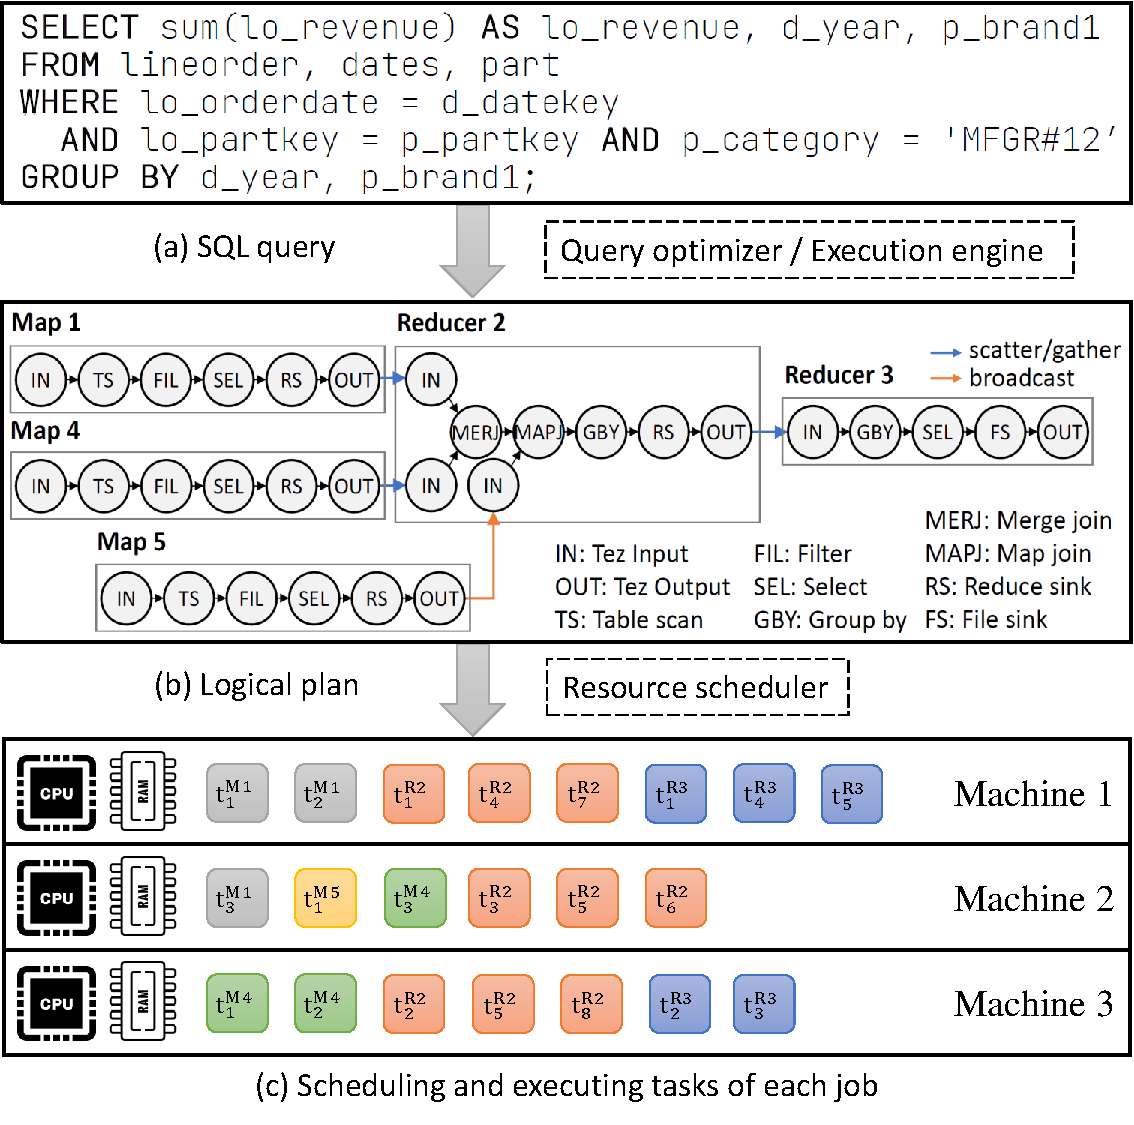
\includegraphics[width=0.40\textwidth]{figures/system/qry_processingvis.pdf}
	\vspace{-3mm}
	\caption{The workflow of distributed query execution in \hive{}}
	\label{fig:qry}
	\vspace{-6mm}
\end{figure}


\autoref{fig:qry} depicts the workflow of query execution in \hive{}.
When a query (e.g., the SQL-like statement in \autoref{fig:qry}(a)) is issued to the system, the query optimizer (e.g., Calcite~\cite{begoli2018apache}) and parallel execution engine (e.g., Tez~\cite{saha2015apache}) optimize and compile the query to a logical execution plan, which is the direct acyclic graph (DAG) of Map/Reducer jobs shown in \autoref{fig:qry}(b).
Each Map or Reducer job in the DAG can be divided into three phases: (1) input, (2) processing, and (3) output.
The input phase loads data from disk or upstream jobs.
The processing phase executes a sequence of SQL operators, for example, the processing phase of Map 1 encompasses three SQL operators: table scan (TS), filter (FIL), and select (SEL).
The output phase generates the output data, which can be the final result or input data for downstream jobs.
The dependencies among the jobs are determined by their input/output relation and modeled by the edges in the DAG.


%, which are the atomic execution units
To run each Map/Reducer job, the execution engine (e.g., Tez) instantiates a set of tasks.
All tasks of a specific Map/Reducer job run the same sequence of operators but work on different data partitions.
For example, the execution engine instantiates three tasks, e.g., $t_{1}[1], t_{1}[2]$, and $t_{1}[3]$ (the gray cells in \autoref{fig:qry}(c)) for job Map 1 in \autoref{fig:qry}(b). 
Each task is scheduled to run on an executor (e.g., container in \hive{}), which is a logical collection of physical resources (e.g., CPU and memory) on one machine in the cluster, by the resource scheduler (e.g., Yarn~\cite{vavilapalli2013apache}).
%Specifically, task is the atomic scheduling unit of a SQL query.
% In addition, different tasks of different jobs can be executed by the same container, i.e., the physical machine.
Task is the atomic unit for execution and scheduling, and the tasks of different jobs can run on the same machine.
For example, as illustrated in \autoref{fig:qry}(c), both $t_{1}[1]$ (a task of Map 1) and $t_{2}[1]$ (a task of Reducer 2) are executed on Machine 1. 

%\qm{
%Based on the workflow shown as \autoref{fig:qry}, existing research works perform the study on visualizing query logic (\autoref{fig:qry}(a)), optimization plan (\autoref{fig:qry}(b)) and execution progress (\autoref{fig:qry}(c)) which will be elaborated in \autoref{sec:relexecution}.
%The research works analyzing the query logic and optimization plan can help analysts diagnose the query logic bugs or optimization bugs. 
%Specifically, \qevis{} is orthogonal to these works and target on diagnosing the query execution trace on the distribution environment. \qevis{} can help to analyze the performance issues caused by hardwares. 
%}

\qm{
%	Building upon the workflow depicted in \autoref{fig:qry}, many research primarily focuses on visualizing query logic (\autoref{fig:qry}(a)) and optimization plans (\autoref{fig:qry}(b)). These research efforts are instrumental in diagnosing query logic bugs or optimization bugs. However, it's important to clarify that \qevis{} is distinct and complementary to these studies. \qevis{} specifically targets the diagnosis of query execution traces (\autoref{fig:qry}(c)) in a distributed environment. \qevis{} is designed to analyze performance issues that may arise due to hardware, providing a unique and necessary perspective in the realm of query execution analysis.
Referring to the workflow in \autoref{fig:qry}, many research work mainly focuses on visualizing query logic (\autoref{fig:qry}(a)) and optimization plans (\autoref{fig:qry}(b)). These studies are very helpful in finding bugs in query logic or optimization. But, it is important to note that \qevis{} is different but complements these studies. \qevis{}  focuses on analyzing query execution traces (\autoref{fig:qry}(c)) in a distributed environment. It is designed to study performance issues that might be caused by the scheduling mechanism, resources, or hardware, etc.
}